\documentclass[landscape]{article}
\usepackage{lmodern}
\usepackage{amssymb,amsmath}
\usepackage{ifxetex,ifluatex}
\usepackage{fixltx2e} % provides \textsubscript
\ifnum 0\ifxetex 1\fi\ifluatex 1\fi=0 % if pdftex
  \usepackage[T1]{fontenc}
  \usepackage[utf8]{inputenc}
\else % if luatex or xelatex
  \ifxetex
    \usepackage{mathspec}
  \else
    \usepackage{fontspec}
  \fi
  \defaultfontfeatures{Ligatures=TeX,Scale=MatchLowercase}
\fi
% use upquote if available, for straight quotes in verbatim environments
\IfFileExists{upquote.sty}{\usepackage{upquote}}{}
% use microtype if available
\IfFileExists{microtype.sty}{%
\usepackage{microtype}
\UseMicrotypeSet[protrusion]{basicmath} % disable protrusion for tt fonts
}{}
\usepackage[margin=1in]{geometry}
\usepackage{hyperref}
\hypersetup{unicode=true,
            pdfborder={0 0 0},
            breaklinks=true}
\urlstyle{same}  % don't use monospace font for urls
\usepackage{graphicx,grffile}
\makeatletter
\def\maxwidth{\ifdim\Gin@nat@width>\linewidth\linewidth\else\Gin@nat@width\fi}
\def\maxheight{\ifdim\Gin@nat@height>\textheight\textheight\else\Gin@nat@height\fi}
\makeatother
% Scale images if necessary, so that they will not overflow the page
% margins by default, and it is still possible to overwrite the defaults
% using explicit options in \includegraphics[width, height, ...]{}
\setkeys{Gin}{width=\maxwidth,height=\maxheight,keepaspectratio}
\IfFileExists{parskip.sty}{%
\usepackage{parskip}
}{% else
\setlength{\parindent}{0pt}
\setlength{\parskip}{6pt plus 2pt minus 1pt}
}
\setlength{\emergencystretch}{3em}  % prevent overfull lines
\providecommand{\tightlist}{%
  \setlength{\itemsep}{0pt}\setlength{\parskip}{0pt}}
\setcounter{secnumdepth}{0}
% Redefines (sub)paragraphs to behave more like sections
\ifx\paragraph\undefined\else
\let\oldparagraph\paragraph
\renewcommand{\paragraph}[1]{\oldparagraph{#1}\mbox{}}
\fi
\ifx\subparagraph\undefined\else
\let\oldsubparagraph\subparagraph
\renewcommand{\subparagraph}[1]{\oldsubparagraph{#1}\mbox{}}
\fi

%%% Use protect on footnotes to avoid problems with footnotes in titles
\let\rmarkdownfootnote\footnote%
\def\footnote{\protect\rmarkdownfootnote}

%%% Change title format to be more compact
\usepackage{titling}

% Create subtitle command for use in maketitle
\providecommand{\subtitle}[1]{
  \posttitle{
    \begin{center}\large#1\end{center}
    }
}

\setlength{\droptitle}{-2em}

  \title{}
    \pretitle{\vspace{\droptitle}}
  \posttitle{}
    \author{}
    \preauthor{}\postauthor{}
    \date{}
    \predate{}\postdate{}
  
\usepackage{booktabs}
\usepackage{longtable}
\usepackage{array}
\usepackage{multirow}
\usepackage{wrapfig}
\usepackage{float}
\usepackage{colortbl}
\usepackage{pdflscape}
\usepackage{tabu}
\usepackage{threeparttable}
\usepackage{threeparttablex}
\usepackage[normalem]{ulem}
\usepackage{makecell}
\usepackage{xcolor}

\usepackage{setspace}
\doublespacing
\usepackage{lineno}
\usepackage[width=\textwidth]{caption}

\begin{document}

\hypertarget{appendix}{%
\section{Appendix}\label{appendix}}

\begin{table}[!h]

\caption{\label{tab:unnamed-chunk-1}Site description of all the current permanent sampling plots in the greater Yangambi region. We list the forest type, plot number, geographic location (in decimal degrees), stem density, basal area Above Ground Carbon (AGC), species richness and Land-Use and Land-Cover Change (LULCC) classes in a radius of 100m around each plot location.}
\centering
\begin{tabular}[t]{lrrrrrrrl}
\toprule
type & nr & latitude & longitude & stem density ($ha\textsuperscript{-1}$) & basal area ($m\textsuperscript{2}$ $ha\textsuperscript{-1}$) & AGC (Mg C $ha\textsuperscript{-1}$) & species richness & LULCC class coverage (\%)\\
\midrule
fallow & 1 & 0.7959139 & 24.49423 & 350 & 5.39000 & 6.7000 & 26 & 37 (1), 63 (3)\\
fallow & 2 & 0.7921028 & 24.49717 & 132 & 2.06000 & 2.0400 & 22 & 68 (1), 32 (3)\\
young-regrowth & 1 & 0.7894028 & 24.51755 & 322 & 20.44000 & 46.5600 & 40 & 68 (1), 32 (3)\\
young-regrowth & 2 & 0.7948806 & 24.49193 & 447 & 16.63000 & 27.8300 & 25 & 56 (1), 44 (3)\\
young-regrowth & 3 & 0.7931083 & 24.49013 & 313 & 17.80000 & 37.1000 & 43 & 51 (1), 49 (3)\\
\addlinespace
old-regrowth & 1 & 0.8824444 & 24.49614 & 384 & 19.48000 & 81.7800 & 92 & 100 (1)\\
mixed & 1 & 0.8135486 & 24.51264 & 563 & 34.81000 & 168.0400 & 83 & 100 (1)\\
mixed & 2 & 0.7805000 & 24.52109 & 403 & 35.25000 & 174.5800 & 78 & 100 (1)\\
mixed & 3 & 0.7866181 & 24.52349 & 367 & 30.69000 & 150.3000 & 75 & 100 (1)\\
mixed & 4 & 0.8140333 & 24.49370 & 432 & 33.01000 & 168.6100 & 84 & 100 (1)\\
\addlinespace
mixed & 5 & 0.8025611 & 24.48750 & 329 & 25.20000 & 124.1800 & 80 & 100 (1)\\
mixed & 6 & 0.9925556 & 24.53906 & 490 & 32.63000 & 203.8100 & 86 & 100 (1)\\
mixed & 7 & 0.9898056 & 24.53853 & 598 & 31.47000 & 146.1100 & 92 & 100 (1)\\
mixed & 8 & 0.9866111 & 24.53856 & 556 & 29.20000 & 148.2100 & 90 & 100 (1)\\
mono-dominant & 1 & 0.8269306 & 24.52303 & 344 & 31.80000 & 183.0100 & 48 & 100 (1)\\
\addlinespace
mono-dominant & 2 & 0.8282708 & 24.53196 & 436 & 32.06000 & 173.5800 & 55 & 100 (1)\\
mono-dominant & 3 & 0.7965903 & 24.49779 & 376 & 30.57000 & 166.4400 & 62 & 100 (1)\\
mono-dominant & 4 & 0.8080889 & 24.52811 & 374 & 27.69000 & 145.5500 & 46 & 100 (1)\\
mono-dominant & 5 & 0.8682806 & 24.45655 & 217 & 27.19000 & 159.0000 & 46 & 95 (1), 5 (2)\\
mono-dominant & 6 & 0.7992278 & 24.49195 & 378 & 33.95000 & 165.4800 & 68 & 100 (1)\\
\addlinespace
edge & 1 & 0.7895486 & 24.51990 & 415 & 30.93601 & 152.2792 & 77 & 100 (1)\\
edge & 2 & 0.7979472 & 24.48885 & 368 & 31.82097 & 152.1736 & 72 & 95 (1), 5 (3)\\
edge & 3 & 0.8144250 & 24.48555 & 458 & 35.79959 & 197.4022 & 86 & 100 (1)\\
edge & 4 & 0.7659306 & 24.51125 & 320 & 29.72547 & 154.6380 & 75 & 98 (1), 2 (3)\\
edge & 5 & 0.8691778 & 24.47019 & 459 & 33.72462 & 158.6934 & 88 & 100 (1)\\
\bottomrule
\end{tabular}
\end{table}

\begin{table}[!h]

\caption{\label{tab:unnamed-chunk-2}Flight path meta-data for the Isangi-Stanleyville aerial survey. Data provided consists of the flight path number, cardinal direction of the flight, the image numbers, and the duration of the flight provided by the start and end time of the acquisition. Data is sourced from Appendix Figure 2 and the sensor logs recorded in the margin of acquired images (see Figure 1 main manuscript).}
\centering
\begin{tabular}[t]{rllll}
\toprule
path & direction & image \# & start (H:M:S) & end (H:M:S)\\
\midrule
1 & W – E & 04 / 78 – 04 / 127 & 10:15:00 & 10:40:00\\
2 & W – E & 05 / 01 – 05 / 56 & 10:15:00 & 10:40:00\\
3 & W – E & 06 / 01 – 06 / 48 & 08:55:00 & 09:20:00\\
4 & W – E & 07 / 01 – 07 / 20 & 09:30:00 & 09:45:00\\
5 & W – E & 05 / 167 – 05 / 187 & 08:55:00 & 09:10:00\\
\addlinespace
6 & W – E & 07 / 67 – 07 / 82 & 10:50:00 & 11:00:00\\
7 & E – W & 06 / 49 – 06 / 95 & 09:35:00 & 10:05:00\\
8 & E – W & 05 / 57 – 05 / 103 & 10:20:00 & 10:50:00\\
9 & E – W & 04 / 128 – 04 / 176 & 10:50:00 & 11:10:00\\
10 & W – E & 08 / 01 – 08 / 27 & 09:05:00 & 09:20:00\\
\addlinespace
11 & W – E & 06 / 96 – 06 / 139 & 10:25:00 & 10:45:00\\
\bottomrule
\end{tabular}
\end{table}

\pagebreak

\begin{figure}
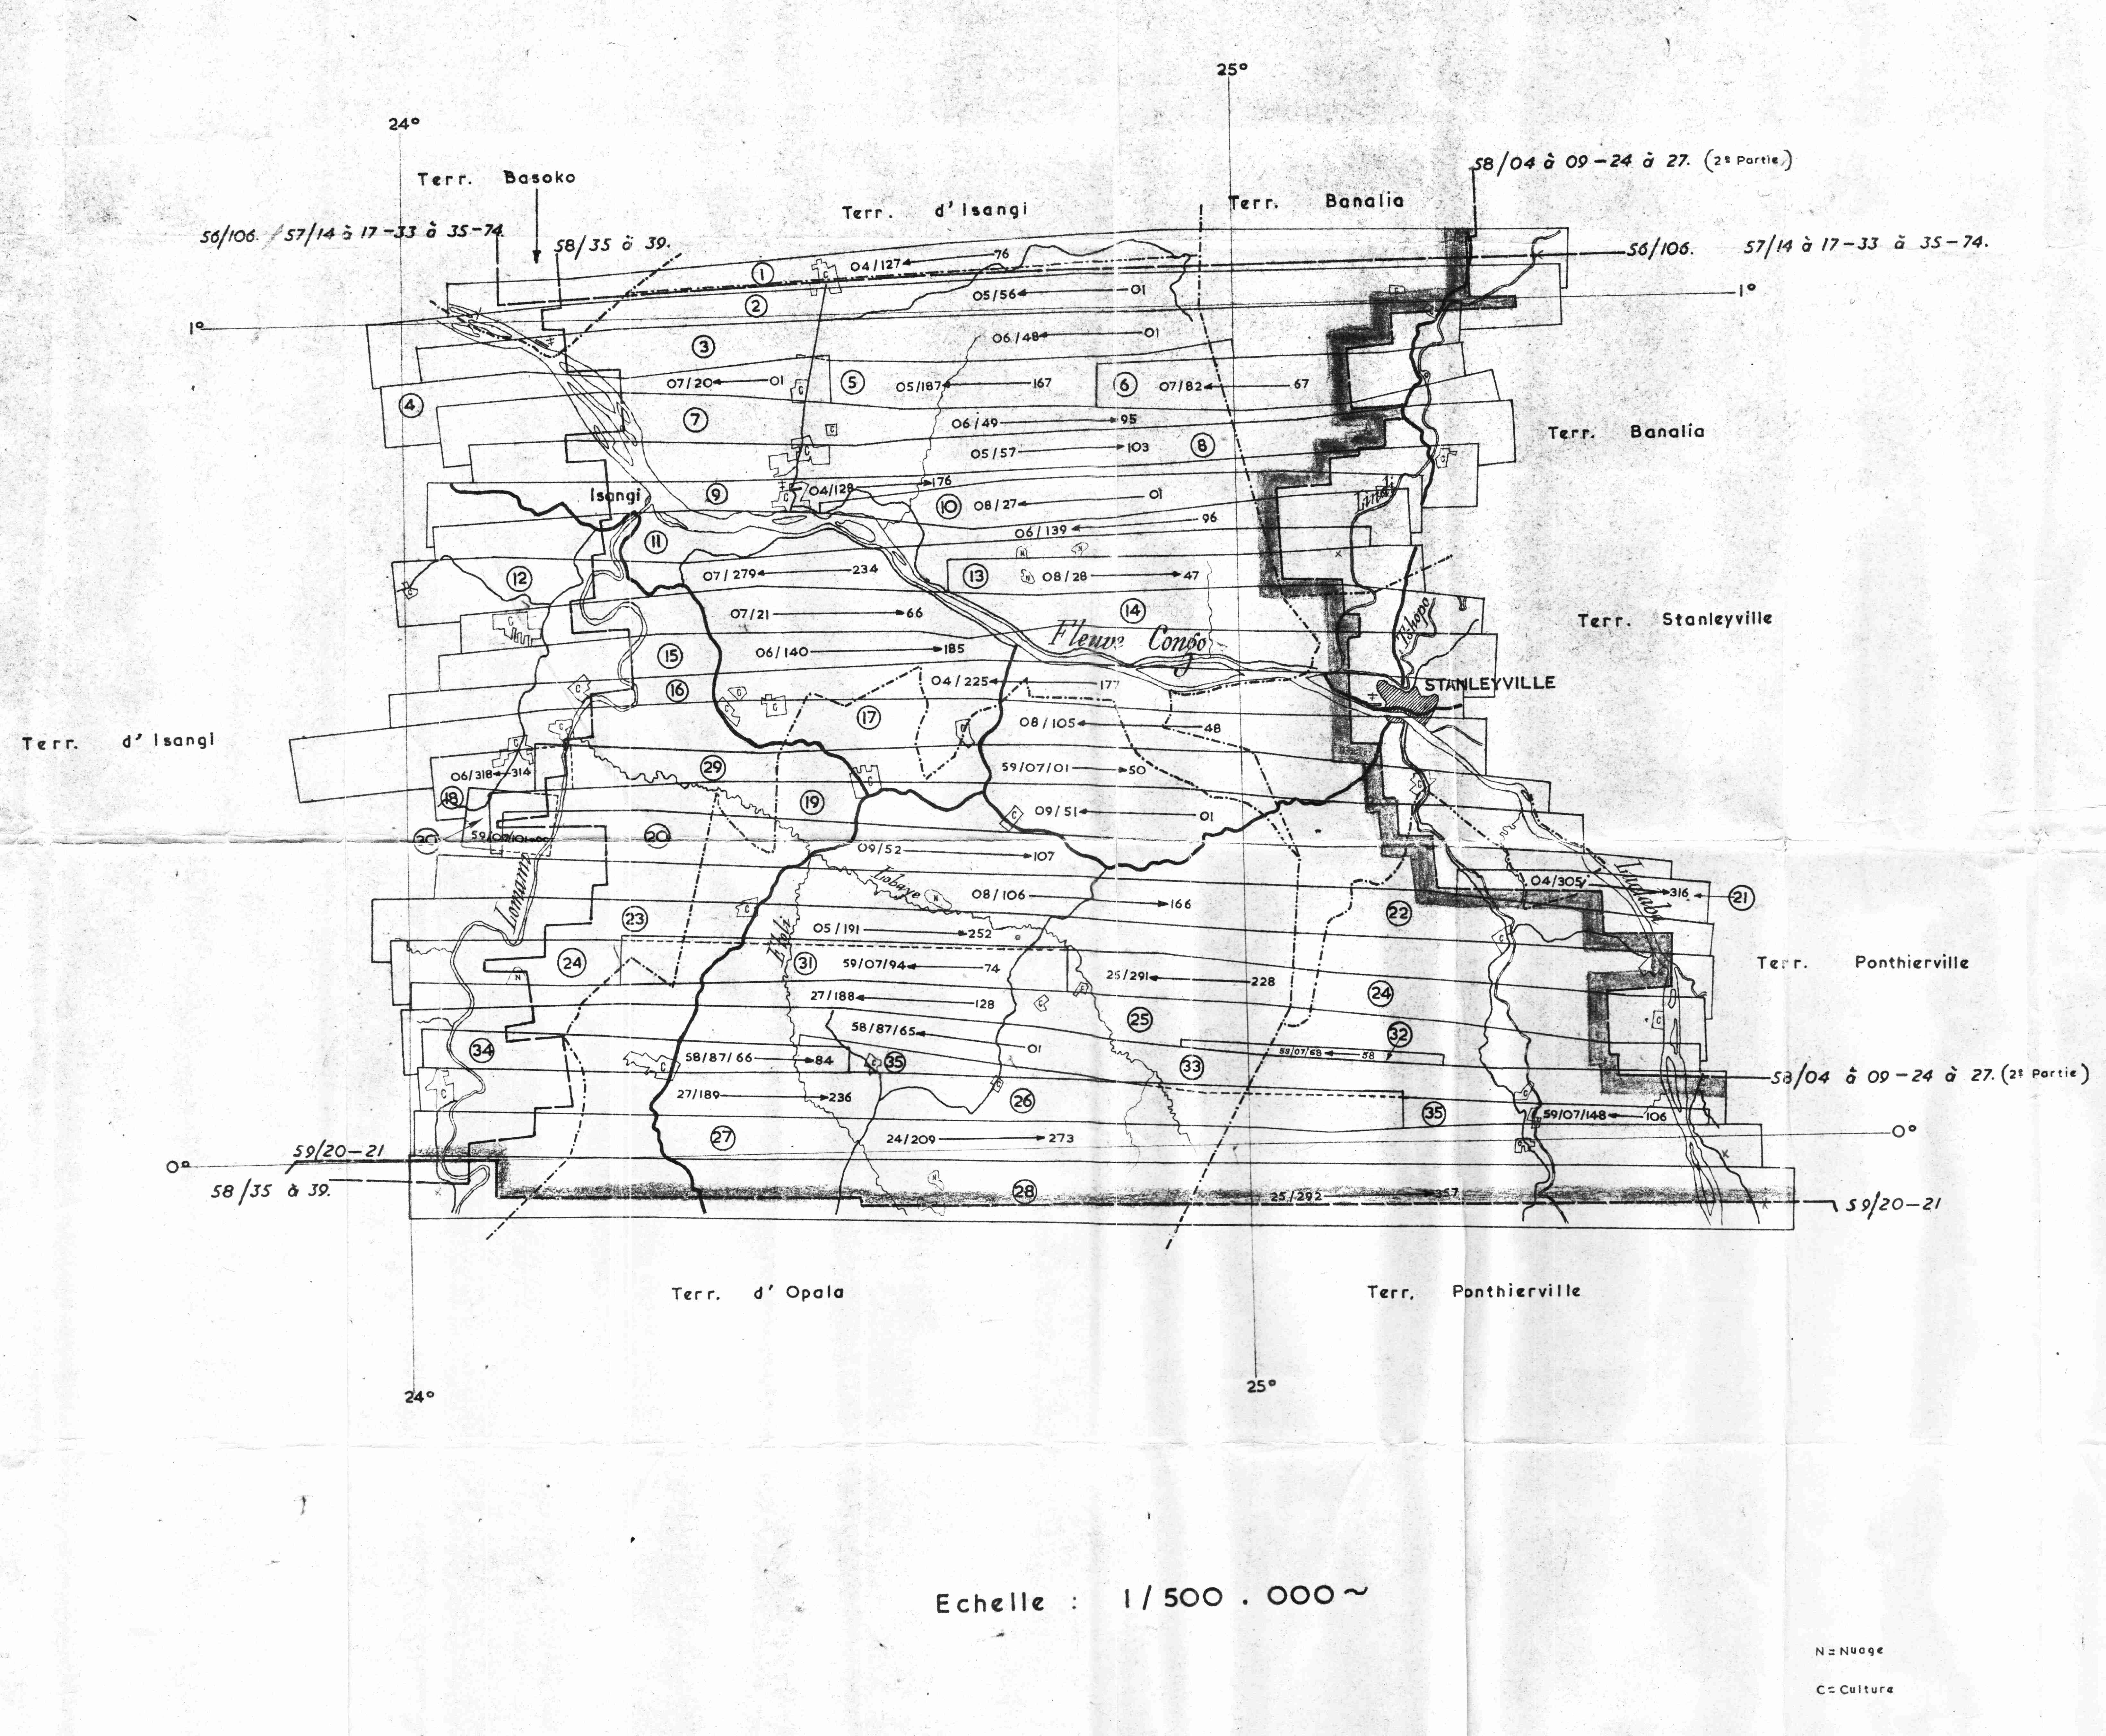
\includegraphics[width=1\linewidth]{./figures/flight_paths_overview} \caption{Overview of the complete flight plan of the survey around Kisangani (then Stanleyville) stored in the archives at the Africa Museum.}\label{fig:unnamed-chunk-3}
\end{figure}

\pagebreak

\begin{figure}
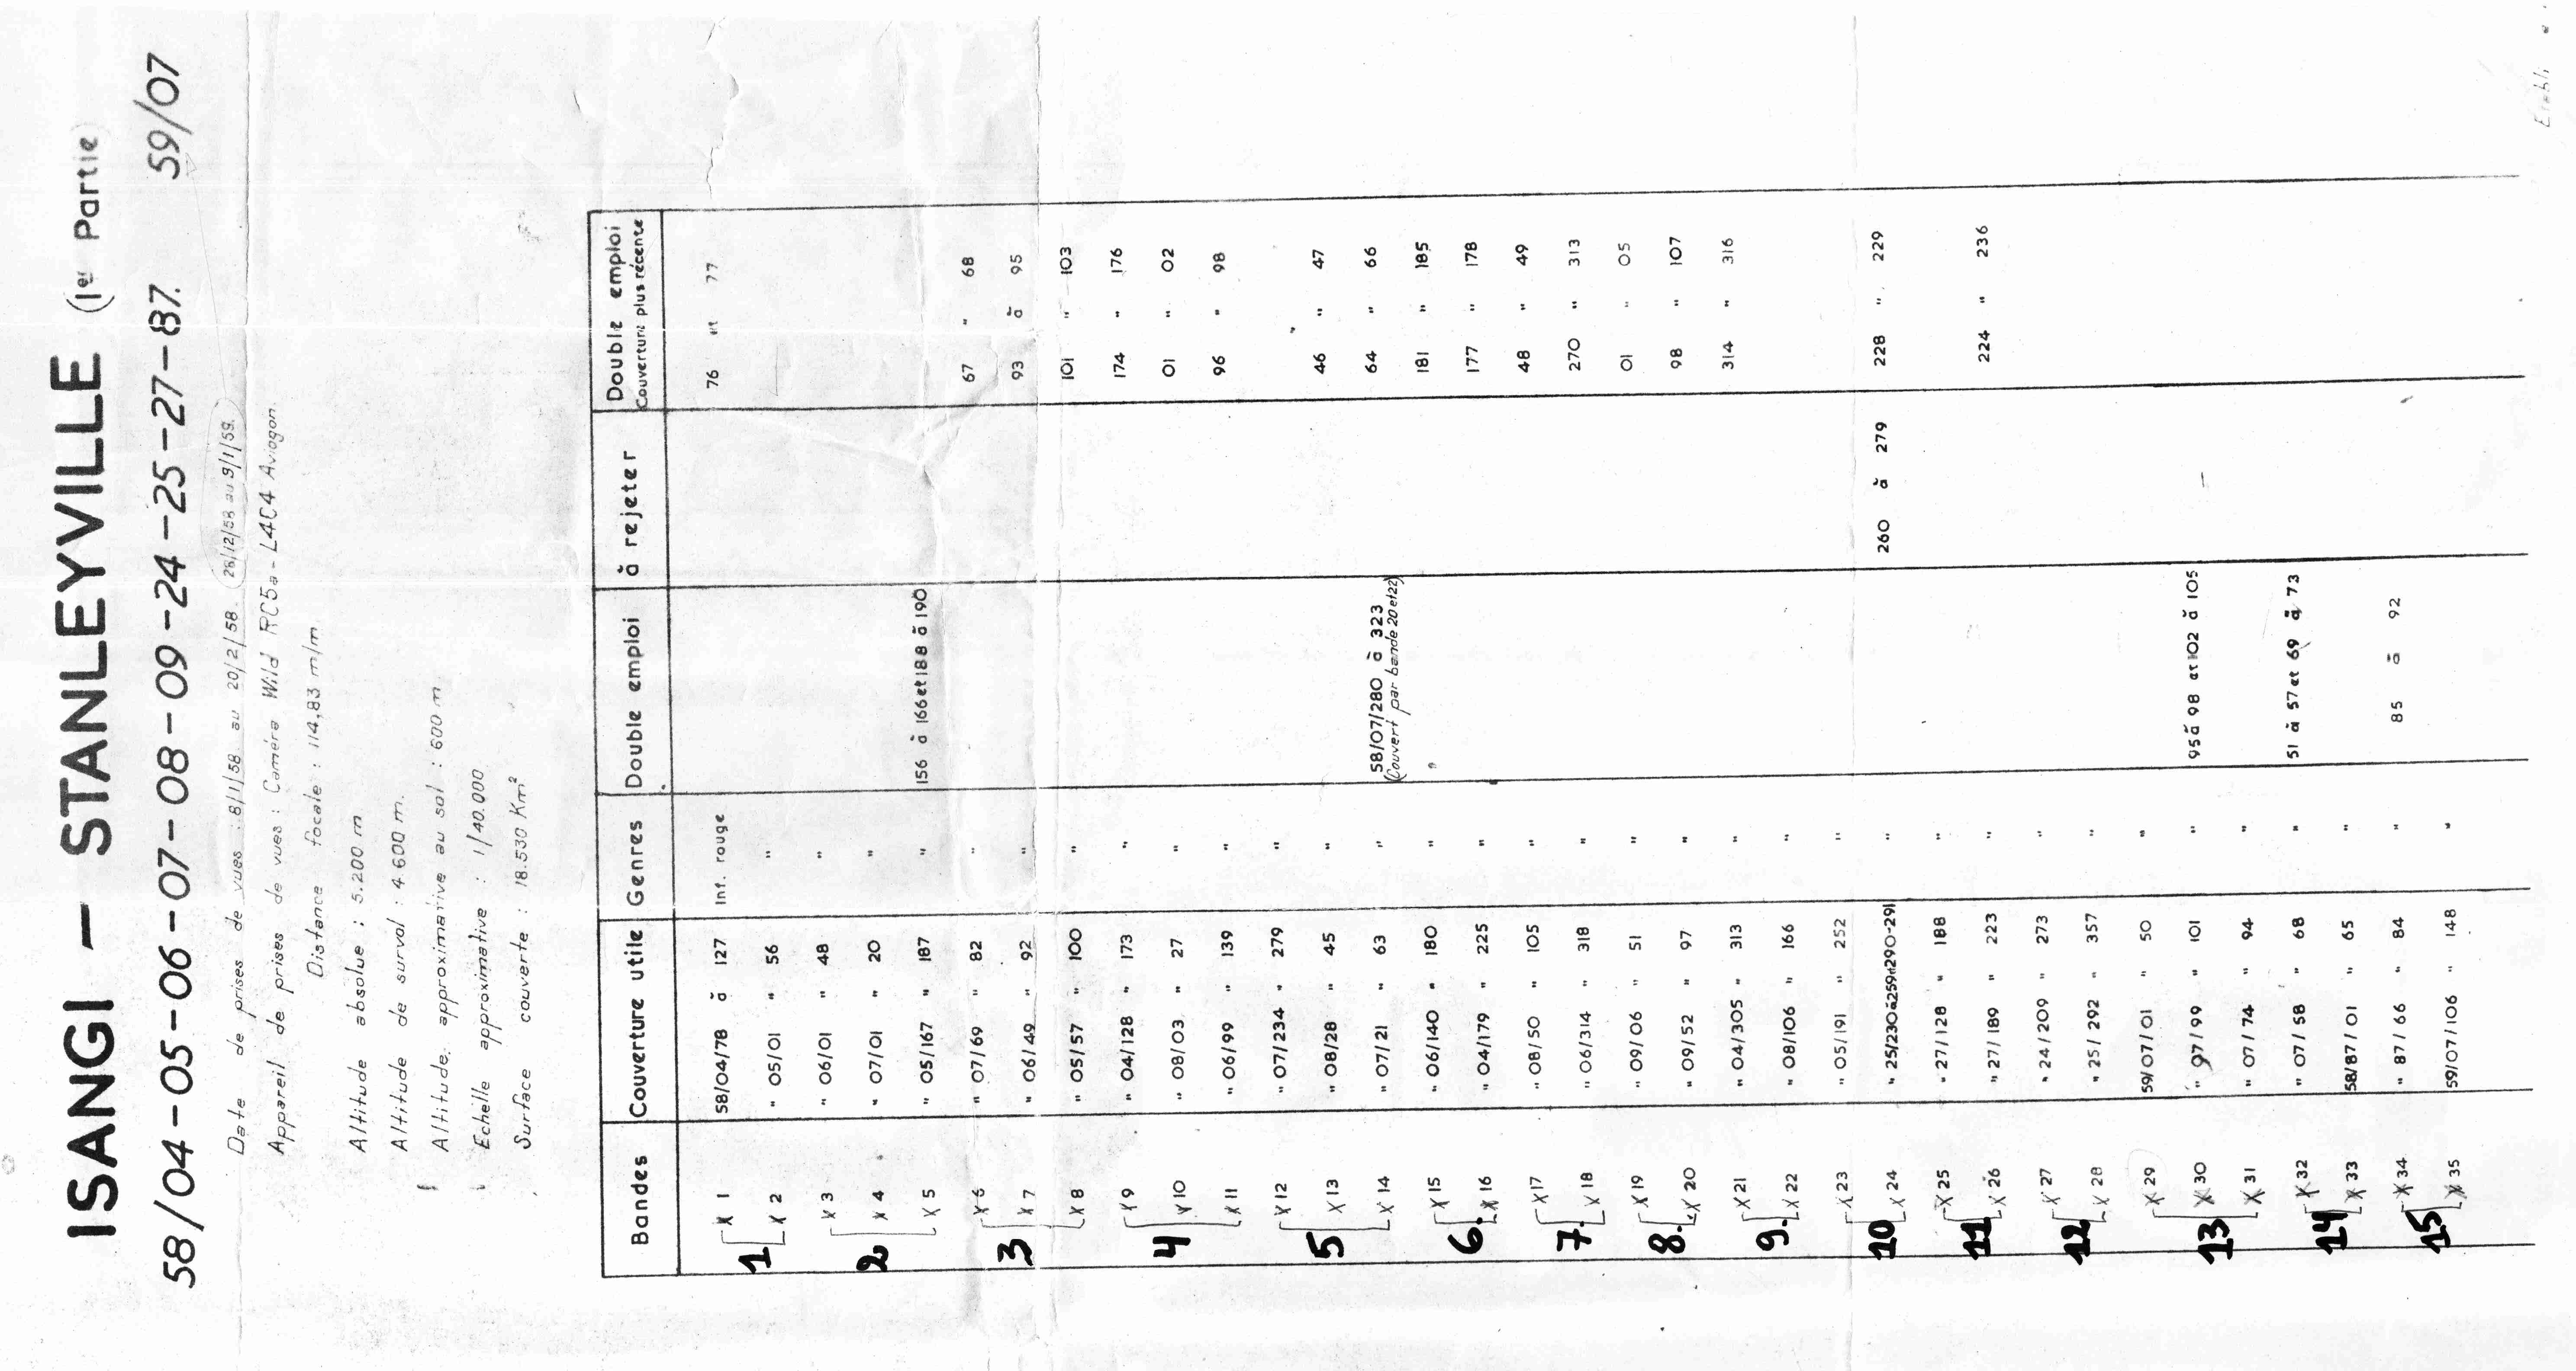
\includegraphics[height=0.75\textheight]{./figures/flight_paths_meta_data} \caption{Overview of the complete flight plan meta-data as stored in the archives at the Africa Museum.}\label{fig:unnamed-chunk-4}
\end{figure}

\pagebreak

\begin{figure}
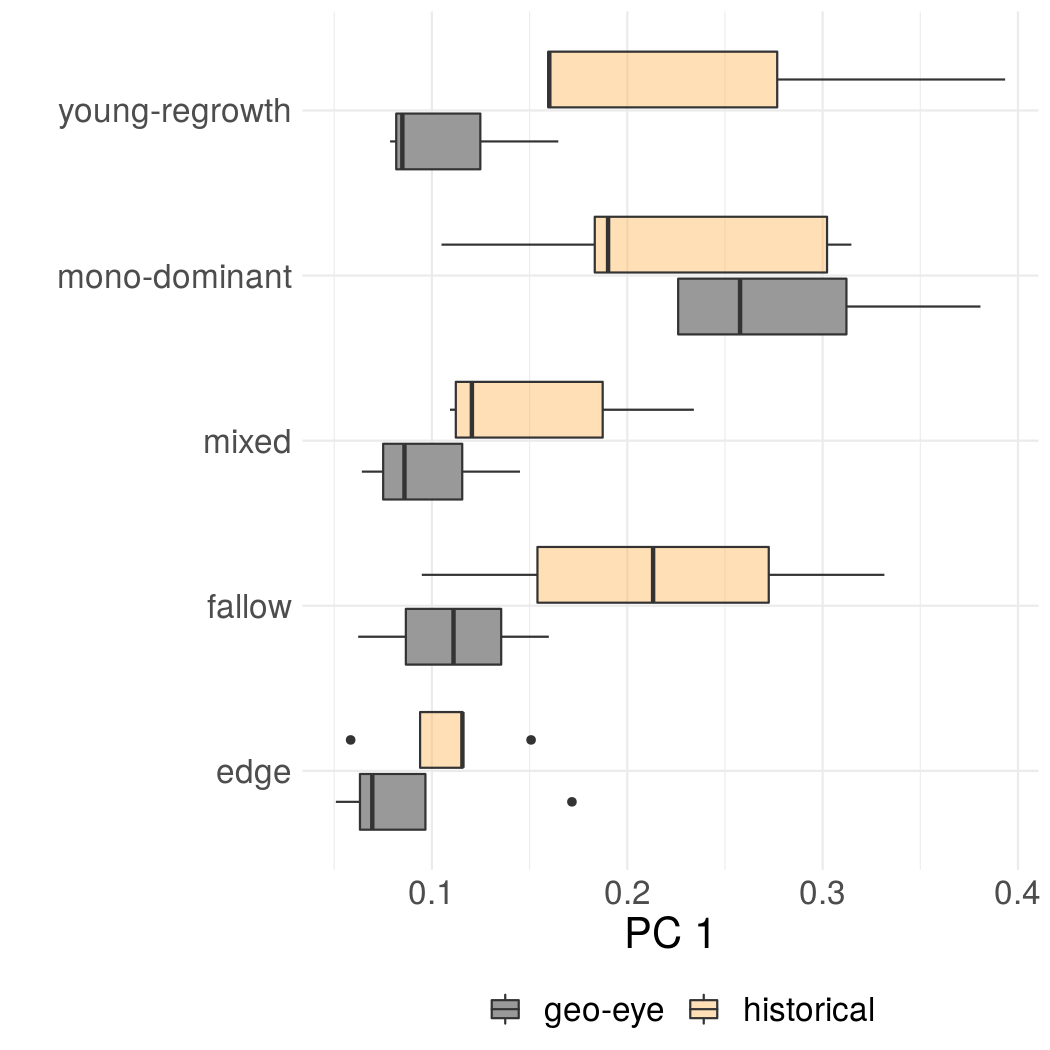
\includegraphics[width=14.58in,height=0.5\textheight]{./figures/foto_bplot_psp} \caption{Boxplots comparing the first principal component (PC1) of a site based FOTO analysis across different forest types for both contemporary (Geo-Eye) and historical orthomosaic data.}\label{fig:unnamed-chunk-5}
\end{figure}

\begin{figure}
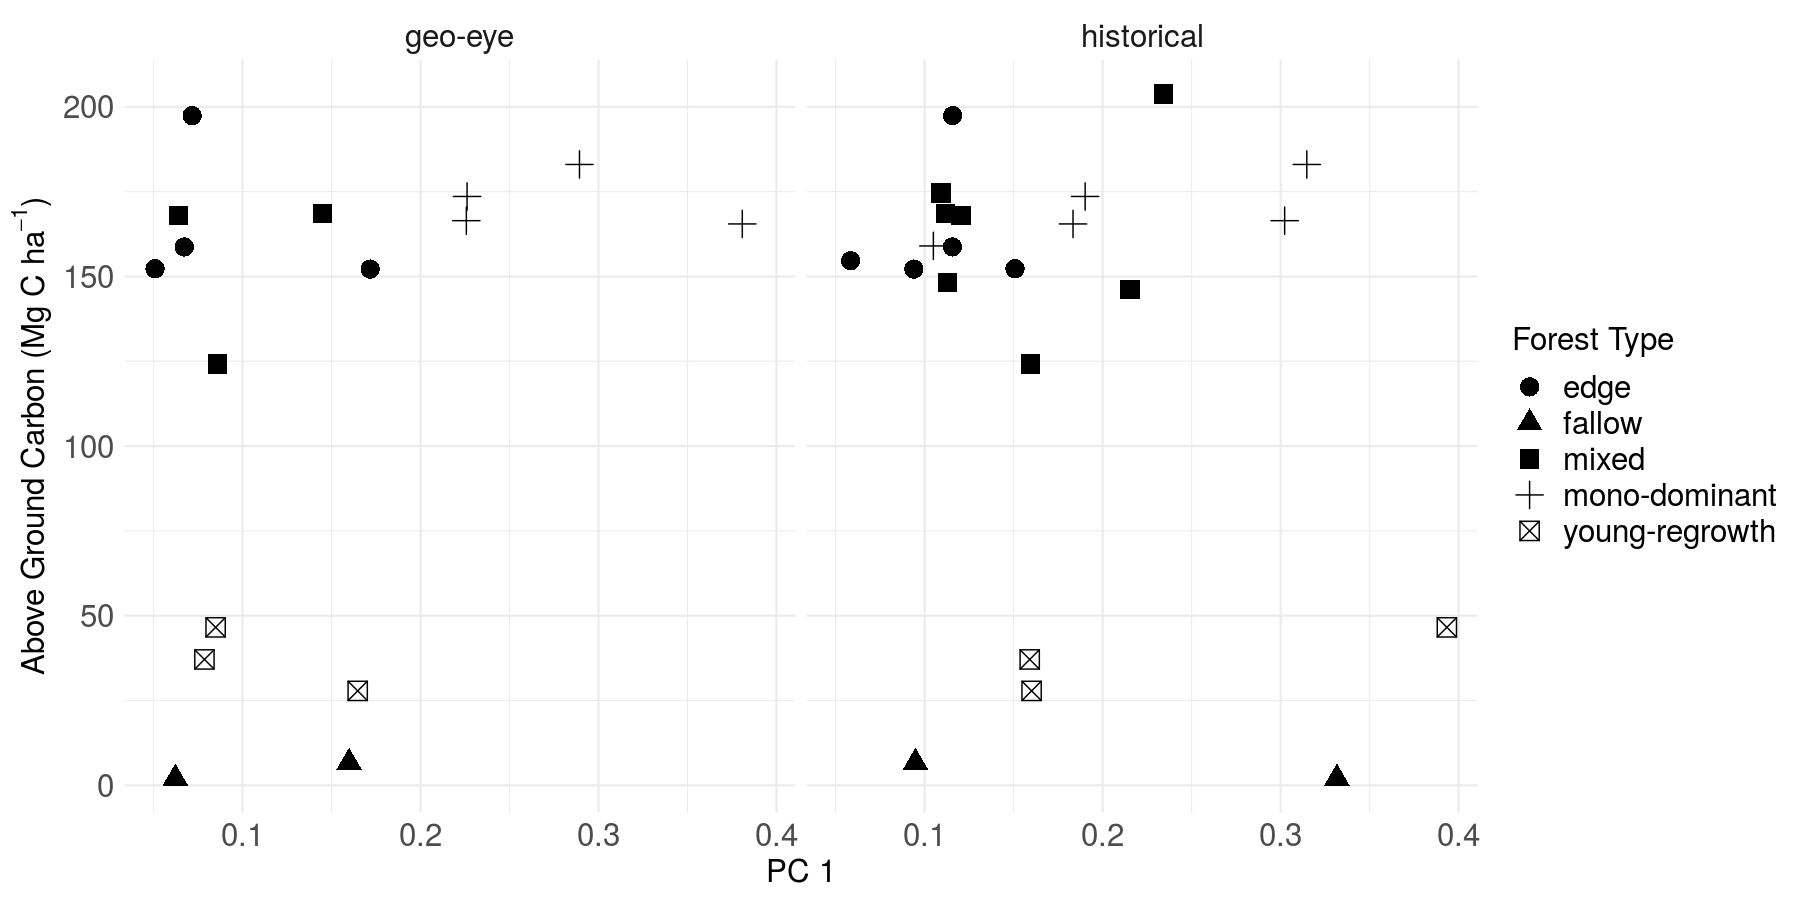
\includegraphics[width=0.75\linewidth]{./figures/foto_pc1_agc} \caption{Scatterplot comparing Above Ground Carbon and the first principal component of the FOTO analysis for contemporary Geo-Eye (left) and the historical orthomosaic (right) data. Different forest types are plotted using closed circles, closed triangles, closed squares and this for fallow, mixed mon-dominant and young-regrowth forests, respectivelly }\label{fig:unnamed-chunk-6}
\end{figure}

\begin{figure}
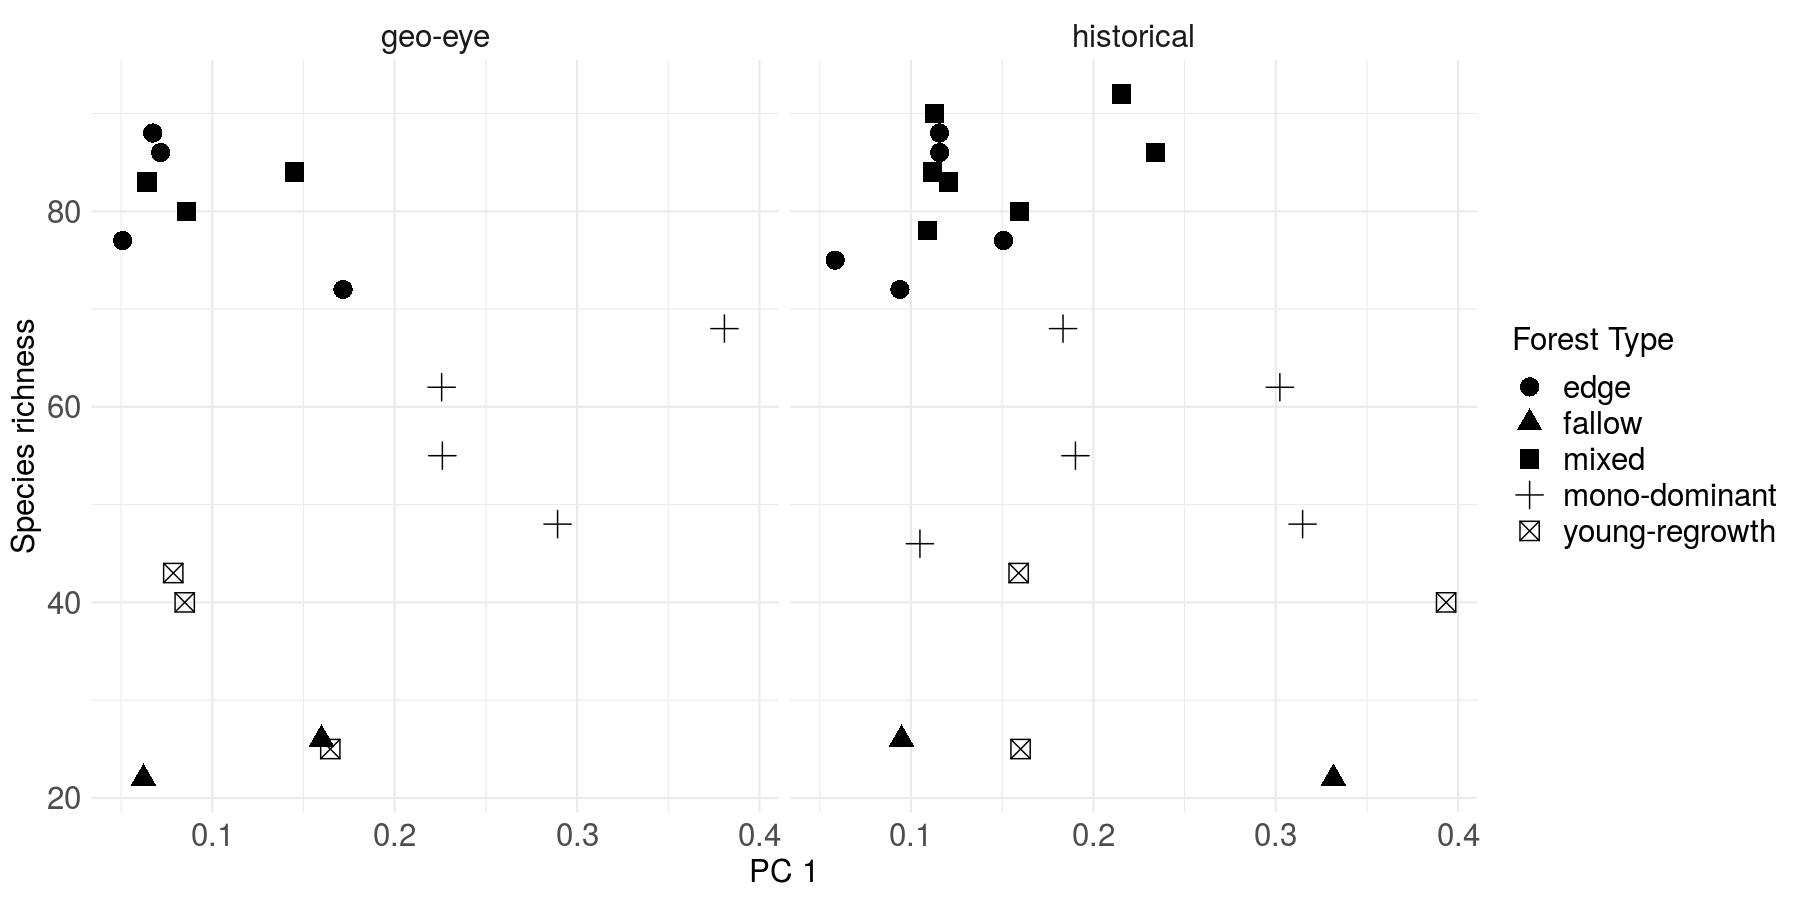
\includegraphics[width=0.75\linewidth]{./figures/foto_pc1_diversity} \caption{Scatterplot comparing tree species richness and the first principal component of the FOTO analysis for contemporary Geo-Eye (left) and the historical orthomosaic (right) data. Different forest types are plotted using closed circles, closed triangles, closed squares and this for fallow, mixed mon-dominant and young-regrowth forests, respectivelly}\label{fig:unnamed-chunk-7}
\end{figure}

\begin{figure}
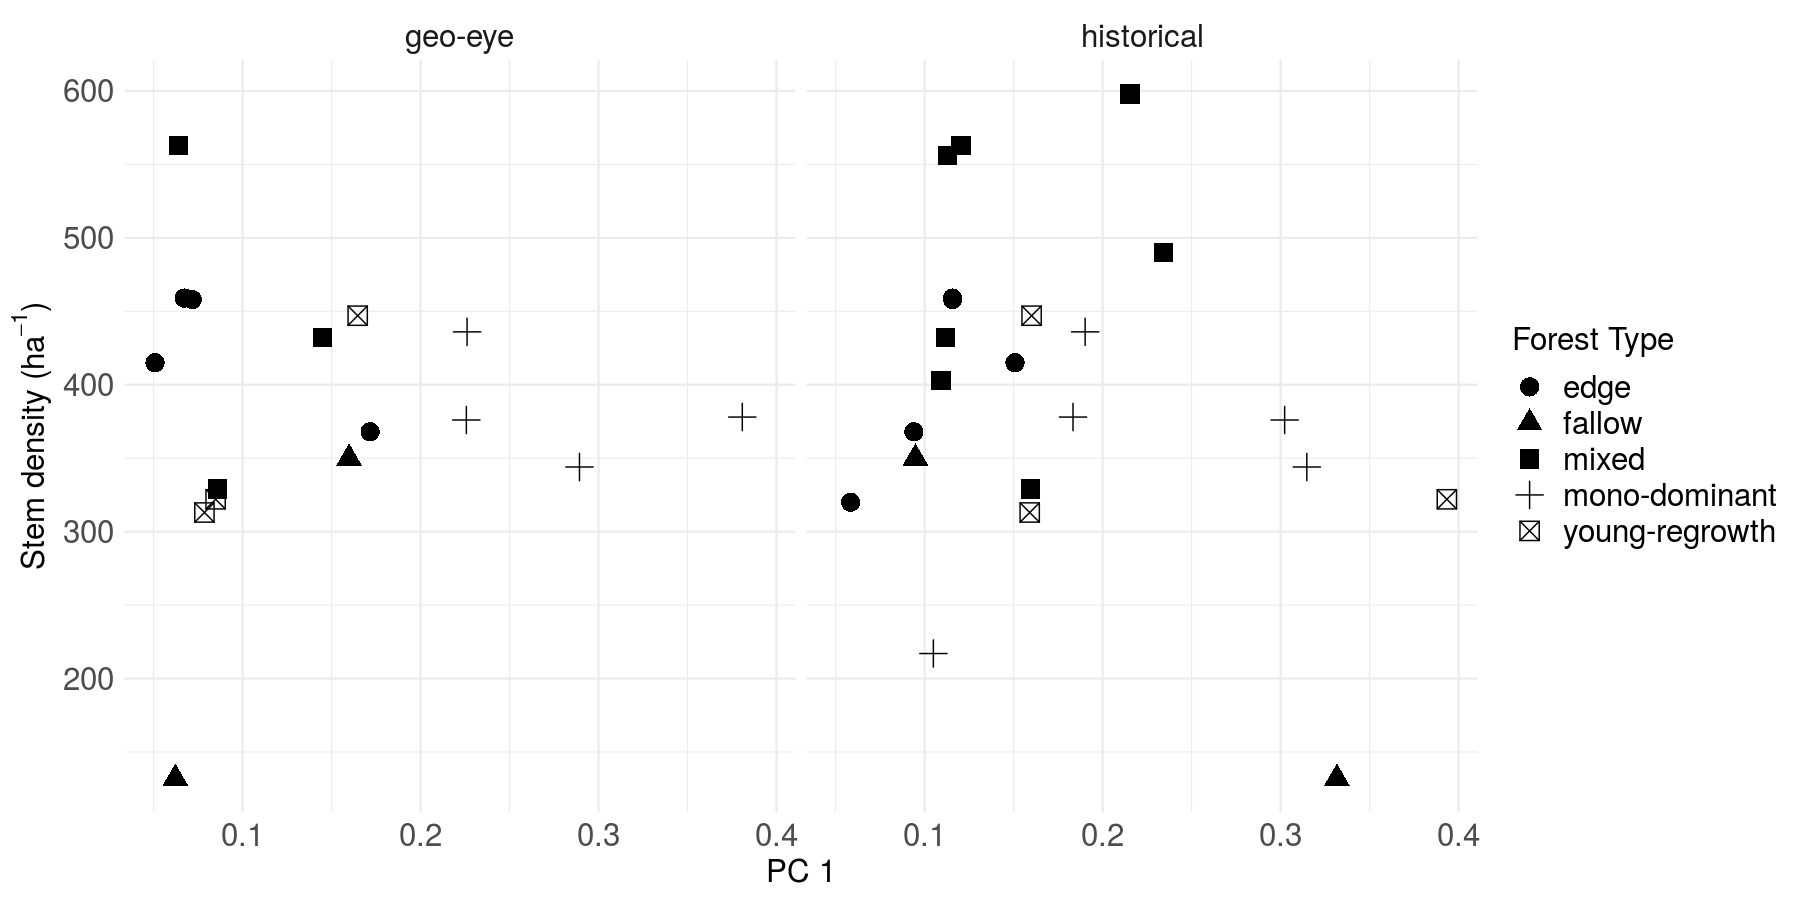
\includegraphics[width=0.75\linewidth]{./figures/foto_pc1_stems} \caption{Scatterplot comparing stem density (per ha) and the first principal component of the FOTO analysis for contemporary Geo-Eye (left) and the historical orthomosaic (right) data. Different forest types are plotted using closed circles, closed triangles, closed squares and this for fallow, mixed mon-dominant and young-regrowth forests, respectivelly}\label{fig:unnamed-chunk-8}
\end{figure}

\pagebreak

\begin{figure}
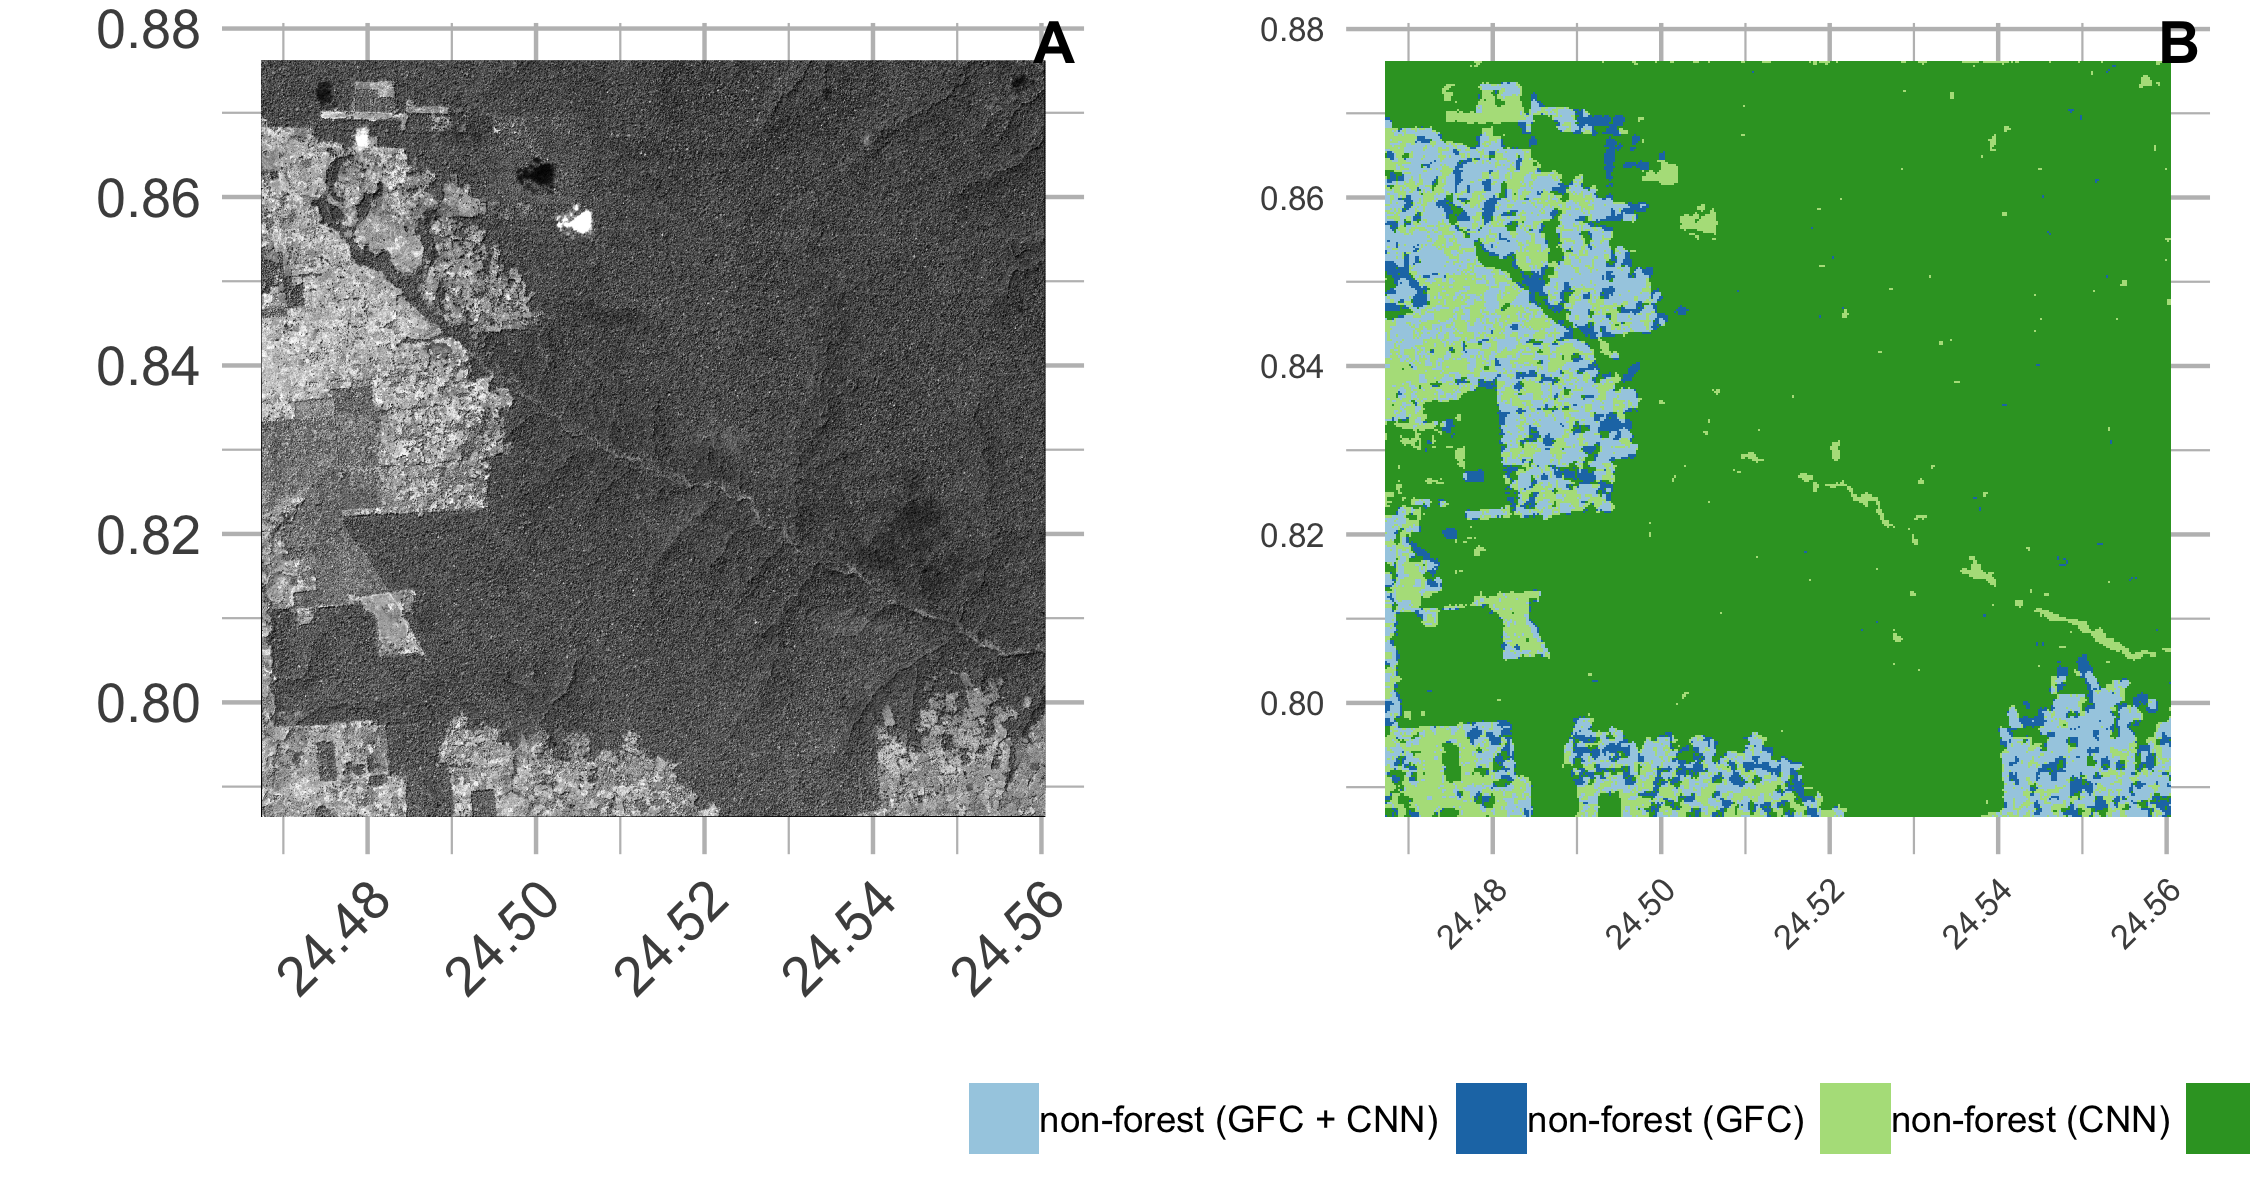
\includegraphics[width=31.25in,height=0.75\textheight]{./figures/visual_comparison_classifiers} \caption{CNN classifier results as run on a recent (2012) Geo-Eye panchromatic image. Results are compared with the Landsat based .}\label{fig:unnamed-chunk-9}
\end{figure}

\begin{table}[!h]

\caption{\label{tab:unnamed-chunk-10}Contingency table between the two forest / non-forest maps generated from a Geo-Eye 1 pan-chromatic image using a Convolutional Neural Network (CNN) generated and the Global Forest Cover map (Hansen et al. 2013).}
\centering
\begin{tabular}[t]{lrr}
\toprule
\multicolumn{1}{c}{CNN} & \multicolumn{2}{c}{Global Forest Cover} \\
\cmidrule(l{3pt}r{3pt}){1-1} \cmidrule(l{3pt}r{3pt}){2-3}
  & non-forest & forest\\
\midrule
non-forest & 0.10 & 0.09\\
forest & 0.04 & 0.77\\
\bottomrule
\end{tabular}
\end{table}


\end{document}
